\documentclass[a4paper, 12pt]{skthesis}
\usepackage{lgrind}
\usepackage{cmap}
\usepackage{mathtools}

\usepackage{amssymb}
\usepackage{float}
\usepackage{braket}
\usepackage[
backend=bibtex,
sorting=none,
style=phys
]{biblatex}
\bibliography{biblio}
%\addbibresource{biblio.bib}
%\usepackage[T2A]{fontenc}
\newcommand{\li}{\mathrm{Li}\,}
\newcommand{\wf}[2]{\psi_{\mathrm{#2}}^{\mathrm{#1}}}
\newcommand{\medium}{medium}
\newcommand{\verylong}{longest}

\begin{document}
	

%% Everything with --rus inside is supposed to be written in russian

\title{Topological Josephson Tunnel junctions}
\titlerus{Туннельные топологические джозефсоновские контакты}

\author{Anton Naumov}
\authorrus{Наумов Антон}

\department{Theoretical and mathematical physics}
\departmentrus{Теоретическая и математическая физика}

\degree{Master of Physics}
\degreerus{Магистр}

\degreemonth{May}
\degreeyear{2019}
\thesisdate{May 31, 2019}
\degreemonthrus{Май}
\thesisdaterus{Май 31, 2019}

\supervisor{Pavel Ioselevich}{Associate Professor}{PhD in Theoretical physics, Doctor of science}
\cosupervisor{Mikhail Skvortsov}{Associate Professor}{Professor}

\supervisorrus{Павел Иоселевич}{Профессор}{Кандидат физ.-мат. наук}
\cosupervisorrus{Михаил Сковрцов}{Профессор}{Доцент}

%\chairman{Arthur C. Smith}{Chairman, Department Committee on Graduate Theses}


\maketitle
\rusmaketitle

\setcounter{savepage}{\thepage}
\begin{abstractpage}
Topological superconductivity is relatively fresh topic of condensed matter physics. Being a rich platform for intriguing and beautiful problems, it also has a huge and unrevealed potential for technology, especially for quantum computing.

The notion of topological superconductivity is closely related to a possibility of presence of a Majorana state --- special topologically protected state, usually localized near some inhomogeneity in a topological superconductor. Despite  the numerous theoritical proposals of construction this state in condensed matter, little experimental signatures of them are obtained.

In this work the system of two one-dimensional superconducting wires connected with a tunnel junction is considered. Under special conditions this system can host a Majorana fermion. The properties of this system, such as supgap states, stationary supercurrent and ionization under  oscillating external voltage are studied. The results of this work have the potential in developing a new technique of detecting Majorana fermions in such systems.

\end{abstractpage}

% \setcounter{page}{\thesavepage}
 %\begin{abstractpagerus}
% Топологическая сверхпроводимость является относительно новой областью современной физики. Являясь богатым полем для красивых теоретических задач, она также имеет огромный и нереализованный потенциал для использования в практических целях, в особенности для квантовых вычислений


Понятие топологической сверхпроводимости тесно связано с существованием Майорановского состояния --- особенного топологически защищенного квантового состояния, обычно локализованного вблизи некоторой неоднородности в топологическом сверхпроводнике. Несмотря на многочисленные теоретические предложения по созданию этого состояния в твердых телах, его экспериментальное наблюдение все ещё остается сложной и неразработанной задачей

В этой работе рассмотрена система, состоящая из двух одномерных сверхпроводников, соединенных туннельным контактом. При определенных условиях такая сисемта может иметь Майрановскоое состояние, локализованное вблизи барьера. В работе изучено наличие подщелевых состояний стационарный сверхток и ионизация под действием внешнего непрерывного излучения. Ответы, полученные в ходе выяснения данных вопросов, имеют потенциальное применение для детектирования Майорановских состояний в подобных системах.
 %\end{abstractpagerus}


%\section*{\centering Acknowledgments}

%This is the acknowledgements section.  You should replace this with your
%own acknowledgements.

%%%%%%%%%%%%%%%%%%%%%%%%%%%%%%%%%%%%%%%%%%%%%%%%%%%%%%%%%%%%%%%%%%%%%%
% -*-latex-*-
 % Your title pages, abstracts and acknowledgments
\include{chapters/contents} % Probably you don't need to change it
%% This is an example first chapter.  You should put chapter/appendix that you
%% write into a separate file, and add a line \include{yourfilename} to
%% main.tex, where `yourfilename.tex' is the name of the chapter/appendix file.
%% You can process specific files by typing their names in at the 
%% \files=
%% prompt when you run the file main.tex through LaTeX.
\chapter{Introduction}


The system considered in this work is a pair of 1D superconductors connected with a Josephson junction. For all the discussion presented it's crucial for one of superconductors to be topological. 

Topological superconductivity is a relatively fresh topic in physics. On the one hand it's connected to particle physics through the notion of Majorana fermion -- the particle coinciding with its own antiparticle \cite{Majorana_1937}. It appears not only in Standard model context 
\cite{particle_majorana_Avignone,
	particle_majorana_Giuliani,
	particle_majorana_Marcocci}
, but also as a state in solids \cite{	majorana_condmat_Rossi,
	majorana_condmat_Kitaev,
	majorana_condmat_Kopnin,
	majorana_condmat_Motrunich,
	majorana_condmat_Nayak,
	majorana_condmat_Read_Green,
	majorana_condmat_Senthil,	majorana_condmat_Volovik,
	majorana_condmat_Fu_Kane,	
	review_majorana_Aguado,	
	review_majorana_Beenakker,
	review_majorana_Oppen}. Despite the difference between these entities, there is a clear analogy between majoranas in condensed matter and majoranas in particle physics \cite{Dirak_BdG_Chamon,Dirak_BdG_Elliott}.

 On the other hand topological superconductivity is of interest to quantum computation community as a platform to build fault tolerant quantum memory \cite{majorana_condmat_Kitaev,quintum_computation_Alicea,quintum_computation_Nayak,quintum_computation_Romito}. Although significant difficulties have appeared on this way, the intention to realize this program is still strong and gives the motivation to build superconducting samples, which demonstrate signatures of nontrivial topology and presence of Majorana fermions \cite{majorana_experiment_Kouwenhoven,majorana_experiment_Vaitiekėnas,majorana_experiment_Zhang}.
 
The proposition of using superconducting wires as carriers of Majorana fermions came from a seminal work of Kitaev \cite{majorana_condmat_Kitaev}. The key ingredient of this system was a p-wave superconductivity assumed to be present in a wire. It was shown, that under certain conditions the Majorana state can be present at the end of the wire. After some time other propositions \cite{Oreg_2010,Lutchyn_2010} appeared, based on seminconductor-superconductor heterostructures with s-wave superconductivity, external magnetic field and spin-orbit coupling. It was showed, that the sign of quantity $ g=B-\sqrt{\Delta^2+\mu^2} $ ( where $ B $ is magnetic field, $ \Delta $ is the absolute value of superconducting order parameter and $ \mu $ is a chemical potential) can be used as a topological index, and a Majorana state will appear where the sign of $g $ is changing.

The model, considered in this work is close to the ones used in \cite{Oreg_2010,Lutchyn_2010}. It consists of two superconducting wires connected with a tunnel junction. However instead of domain wall of the sign of $~g $, a tunnel barrier between areas with $ g>0 $ and $ g<0 $ is introduced. This model is formulated in detail in chapter \ref{chap:model}. The spectrum of this model and stationary supercurrent are studied in chapter \ref{chap:stationary} and the ionization of the Majorana state under small external oscillating voltage is considered in chapter \ref{chap:ionization}. Chapter \ref{chap:discssion}  stands for the discussion of obtained results and their possible experimental realization, while chapter \ref{chap:conclision} concludes the study.



\newcommand{\xbr}{\left(x\right)}
\newcommand{\br}[1]{\left(#1\right)}

\chapter{The model}

The system being under consideration consists of two 1D s-type superconducting wires connected with a tunnel junction. Also  there is a strong spin-orbit coupling assumed to be present and external magnetic field is applied in the direction perpendicular to the wire. The Hamiltonianm of the bulk of each wire, written in the Bogoliubov-de Gennes formalism, is similar to the ones presented in \cite{Oreg_2010} and \cite{Lutchyn_2010}:

\begin{gather}
	\mathcal{H}
	=
	\int dy ~
	\Psi^\dagger
	\br{y}
	H
	\Psi
	\br{y}
	\
	~~~~
	\Psi
%	\left(x\right)
	=
	\begin{pmatrix}
		\psi_\uparrow
		\\
		\psi_\downarrow
		\\
		\psi_\downarrow^\dagger
		\\
		-\psi_\uparrow^\dagger
	\end{pmatrix}
	\\
	\label{bulk_Hamiltonian}
	H
	=
	\br{
		\frac{p^2}{2m}
		-\mu_0
	}\tau_z
	+
	u p \sigma_z \tau_z
	+
	B\sigma_x	
	+
	\Delta\tau_\phi
\end{gather}

Here $ \sigma_i $ and $ \tau_i $ are Pauli matrices in spin and particle-hole subspaces respectfully, $ \tau_\phi = \tau_x \cos\phi - \tau_y \sin_\phi$ with $ \phi $ being a superconducting phase, $ \mu_0 $ is a chemical potential, $ B $ is an external magnetic field, $ \Delta $ is the module of superconducting order parameter and $ u $ is spin-orbit coupling constant with the dimension of velocity. The wire is being aligned along the y-axis, while the direction of the magnetic field coincides with x-axis. Note, that only one component of from spin-orbit is nonzero due to 1D nature of the problem.

The tunnel junction is introduced  by applying an external electrical field. To take it into account it's necessary to include additional term  $ U \br{y}\tau_z $ in (\ref{bulk_Hamiltonian}). However this term can be combined with the chemical potential by introducing $ \mu \br{y} = \mu_0 - U\br{y} $.

\begin{figure}
	\centering
	\includegraphics[width=0.7\linewidth]{images/chem_potential}
	\caption{}
	\label{fig:chempotential}
\end{figure}


It can be argued, that superconducting correlations are not possible in thin wires due to the presence of fluctuations. However in real systems this difficulty can be avoided with the help of the proximity effect. The wire itself is assumed to be metallic or semiconductor, and being put close to a strong superconductor. Due to proximity effect it's possible to obtain a presence of order parameter inside initially nonsuperconducting wire. 
\chapter{Stationary properties} 


\section{Boundary conditions}

To obtain the spectrum of the system it's necessary to find the boundary conditions. As the barrier chemical potential  is the biggest energy parameter of the problem, the wave-functions there are defined by the Hamiltonian:
\begin{gather}
\label{barrier_Hamiltonian}
	H(y)
	=
	\br{
		\frac{p^2}{2m}
		+\mu_b
	}\tau_z,  ~~~~~~~~~-\frac{L}{2}<y<\frac{L}{2}
\end{gather} 

as the low energies are the under consideration, in Sroedinger equation the energy term can be omitted, so $ p_b\approx\pm i \sqrt{2m\mu_b} $. One can solve the problem given by (\ref{barrier_Hamiltonian}) and match the values of the wavefunction and it's derivatives on the left and on the right of the barrier to obtain:
\begin{gather}
	\begin{cases}
	\psi_L + b\partial_y\psi_L=t(\psi_R + b\partial_y\psi_R) \\
	\psi_R - b\partial_y\psi_R=t(\psi_L - b\partial_y\psi_L)
	\end{cases}
\end{gather}

here $ \psi_{L,R}=\psi\br{\mp\frac{L}{2}} $, $ b=\br{{2m\mu_b}}^{-\frac{1}{2}} $ --- the penetration depth for the particle inside th barrier and $ t = e^{-\frac{L}{b} }$ --- the tunneling constant assumed to be small: $ t\ll 1 $. This condition reads, that the size of the barrier $ L $ should be  much bigger that the penetration depth $ b $.

This condition is invariant under the combined action $ L\leftrightarrow R $, $ y\to-y $. To simplify the further analysis one can reverce th direction in the left wire and put both ands of the wires from $ y= \frac{L}{2} $ to $ y=0 $. The boundary condition than becomes:
\begin{gather}
\label{bc_transformed}
\begin{cases}
\psi_L - b\partial_y\psi_L=t(\psi_R + b\partial_y\psi_R) \\
\psi_R - b\partial_y\psi_R=t(\psi_L + b\partial_y\psi_L)
\end{cases}
\end{gather}
This transformation is illustrated on the fig \ref{fig:bctransform}.

The boundary condition (\ref{bc_transformed}) can be rewritten with introducing the spinor $ \Psi=\br{\psi_L, \psi_R}^T $ and Pauli matrices $ s_i $ in LR space:
\begin{gather}
	\br{1-ts_x}\Psi-\br{1+t s_x}b\pdy\Psi=0
\end{gather}
since for all $ t\ne 1 $ (recall, that $ t\ll1 $) the matrix is $ 1\pm ts_x $ in reversible. Multupliing the last equation by $ \br{1-ts_x}/\br{1+t^2} $ one obtain:
\begin{gather}
\label{bc_LR_space}
	\br{1-2\tilde{t}-\tilde{b}\pdy}\psi=0
\end{gather}
where $ \tilde{t}=\frac{t}{1+t^2} $, $ \tilde{b} = \frac{1-t^2}{1+t^2}b $. In the leading order on $ t $, which corresponds to the tunneling limit, $ \tilde{t}=t $, $ \tilde{b} = b $.
\begin{figure}[H]
	\centering
	\includegraphics[width=0.9\linewidth]{images/bc_transform}
	\caption{Illustration of switching the direction of left wire}
	\label{fig:bctransform}
\end{figure}

One can argue, that in tunneling limit the second and the third term in (\ref{bc_LR_space}) are much smaller than the first one and should not be taken when the leading order is considered. However, if the second terms is omitted, the leads become efficiently disconnected, and no tunnel effects can be found. The same is true for the third term --- if it's not present, the boundary condition immediately implies $ \Psi\br{0} = 0 $, so the wires become disconnected again.

\section{High momentum modes}  

As was pointed in section \ref{sec:high_and_low_modes}, there are two  shortwave and longwave wavefunctions inside the wire, and the first ones can be described with the Hamiltonian (\ref{short-long_hamiltonian}). However, if one is looking for the localized states, even the longwave modes should be taken decaying. To obtain this, one needs to add a restore superconducting term in (\ref{short-long_hamiltonian}), so the spectrum become gapped and the momenta can get an imaginary part. So, for shortwave modes one should consider a Hamiltonian:
\begin{gather}
\label{high_mods_hamiltonian}
	H=\br{\frac{p^2}{2m}-ups_z\sigma_z}\tau_z+\Delta\tau_\phi
\end{gather}
here the multiplier $ s_z $ is added in the spin-orbit coupling term, as the direction of the left wire is inverted, so to write a correct Hamiltonian for LR space, one needs to change $ p $ to $ -p $ for the left wire --- which is exactly adding $ -s_z $ multiplier to each momentum.

Denoting $ \eta = \frac{p^2}{2m}-ups_z\sigma_z $, one can rewrite (\ref{high_mods_hamiltonian}) as $ H=\eta\tau_z+\Delta\tau_\phi $. As $ s_z\sigma_z $ commutes with $ H $ one can treat it as a number, so the dispersion is $ E^2 =\eta^2+\Delta^2 $. Thus $ \eta=\pm i\sqrt{\Delta^2-E^2} $, as the case $ \abs{E}<\Delta $ is assumed. For shortwave one can write the equation:
\begin{gather}
	p^2-2mu s_z \sigma_z p - 2m \eta =0
\end{gather}
which for shortwave momenta gives $ p_{short}\approx2 mu s_z \sigma_z + \frac{\eta}{u}s_z\sigma_z$. Choosing the sign of $ \eta $ in a way, that the wavefunction decays at $ x\to \infty $, one can obtain:
\begin{gather}
\label{short_momentum_decaying}
	p_{short}\approx
	2 mu s_z \sigma_z 
	+
	i\frac{\sqrt{\Delta^2-E^2}}{u}
\end{gather}


Now the wavefunction can be constructed by putting (\ref{short_momentum_decaying}) into the Schroedinger equation $ \br{\eta\tau_z +\Delta\tau_\phi}\Psi=E\Psi $. The solutions are:
\begin{gather}
	\Psi_{s_z,\sigma_z}\br{x}
	=
	\begin{pmatrix}
	1
	\\
	e^{i\br{s_z\sigma_z\gamma+\phi_{s_z}}}
	\end{pmatrix}_{eh}
	e^{2imus_z\sigma_zx -\frac{\sqrt{\Delta^2-E^2}}{u}x}
	\ket{s_z, \sigma_z}
\end{gather}
where $ s_z $ and $ \sigma_z $
 should be treated as numbers can be equal $ \pm1 $, $ \ket{s_z, \sigma_z} $ are eigenvectors of matrix $ s_z \sigma_z $ and $ \gamma = -\frac{\pi}{2}+\arcsin\frac{E}{\Delta} $.
Thus the longwave part of eqigenstate can be written as:
\begin{gather}
	\Psi_{long}
	=
	\sum_{s_z=\pm 1}
	\sum_{\sigma_z=\pm 1}
	\Psi_{s_z,\sigma_z}\br{x}
\end{gather}
 
  \if 0
\begin{gather}
\begin{pmatrix}
i s_z \sigma_z\sqrt{\Delta^2-E^2}-E & \Delta e^{-i\phi_{L,R} s_z} \\
\Delta e^{i\phi_{L,R} s_z} & -i s_z \sigma_z\sqrt{\Delta^2-E^2}-E
\end{pmatrix}
\Psi
=
E\Psi
\end{gather}
\fi
and
\chapter{Ionization}

In this chapter the model, previously presented is modified to allow the ionization precesses. The main goal here is to find the ionization rate when the typical size of the photon is much smaller, than the gap int the spectrum.

\section{Introducing the perturbation}

To study the ionization behavior of the system, it's necessary must modify the model considered in chapter \ref{chap:model}. It's reasonable to assume, that this perturbation will be present as an alternating voltage applied to the junction. This may alter the Hamiltonian (\ref{full_hamiltonian}) in two ways --- by the modification of the chemical potentials $ \mu_L, \mu_R $ and by making the superconducting phase difference $ \varphi=\phi_R-\phi_L $ time dependent. The second effect can be described by a Josephson relation:
\begin{gather}
	U\br{t}
	=
	\frac{\hbar}{2e}
	\frac{\partial\varphi\br{t}}{\partial t}
\end{gather}

The ionization voltage is assumed to be small compared to other energy parameters of the system, but this smallness is present in both effects. However, is the frequency $ \omega $ of the voltage is also small, the perturbation induced by the second effect will have additional big multiplier $ \frac{\Delta}{\omega} $ and will be much more important than the. In this chapter only this regime is taken under consideration.

The time dependence of phase difference is introduced as:
\begin{gather}
	\varphi\br{t}=\varphi_0+\alpha\cos\omega t
\end{gather}
where $ \varphi_0 $ is an initial time independent phase difference and $ \alpha $ is an amplitude of phase oscillations.

As was shown in section \ref{sec:elimintaing_longwave}, there exists a gauge transform $ U_\phi $, which may redistribute the phase difference between the wires, so the phase in a given wire can take any value. This ambiguity just reflects a  fact, that only phase difference $ \varphi $ is a observable quantity, but not the phases $ \phi_L $, $ \phi_R $ separately. However when treating the time dependent $ \phi\br{t} $, where the oscillating phase is present. Moreover, the voltage frequency $ \omega $ is assumed to be much smaller than not obly the superconducting gap $ \Delta $, but the spectrum gaps in both wires: $ \omega\ll g_R, \abs{|g_L|} $

\textbf{Pavel's talk about equally disturbed phase}

The correct answer is that both left and right wires should get equal time-dependent phase with different signs: $ \phi_L=-\frac{\varphi_0}{2}-\frac{\alpha}{2}\cos \omega t $, $ \phi_R=\frac{\varphi_0}{2}+\frac{\alpha}{2}\cos \omega t $. Thus the superconducting terms in the wire Hamiltonians alter: $ \Delta_{\pm\frac{\varphi}{2}} \to\Delta_{\pm\frac{\varphi}{2}\pm \frac{\alpha}{2}\cos \omega t} $. Deocmposing them in small $ \alpha $ one can explicitly write the perturbation and try to compute the ionization rate. However this way appears to be quite difficult as the overlaps of all the states 
present in both wires and at first it seems that the Majorana states has to much ways to ionize. To avoid this difficulty, the tunnel Hamiltonian approach is used.
\section{Tunnel Hamiltonian approach}
\label{sec:tunnel_hamiltonian}
The main idea of this method is to hide all the time dependence and the tunnel effect in one single operator. The local goal is to write the Hamiltonian as $ H=H_L+H_R+H_T $ , where $ H_{L,R} $ are the Hamiltonians of the left and right wire without any contact (corresponding to zero tunneling: $ t=0 $), and $H_T  $ is a tunnel Hamiltonain both containing the time dependence and mixing the wavefunctions from different wires. 

Here the following notation is used.The Hamiltonians $ H_L $, $ H_R $ and $ H_T $ are 8x8 matrices in combined Nambu-Gorkov and LR-space. In LR-space they have the following form:
\begin{gather}
	H_L
	=
	\begin{pmatrix}
	h_L & 0 \\
	0 & 0
	\end{pmatrix}_{LR}
	\quad
	H_R
=
\begin{pmatrix}
0 & 0 \\
0 & h_R
\end{pmatrix}_{LR}
\quad
	H_T
=
\begin{pmatrix}
0 & h_T^\dagger \\
h_T & 0
\end{pmatrix}_{LR}	
\end{gather}
 The spinors with four components are corresponding to the unperturbed wavefunctions and are denoted as $ \big|\gamma_{0}\,\big> $,  for the Majorana state and $ \big|\varepsilon,L_{0}\,\big> $, $ \big|\varepsilon,R_{0}\,\big> $ for the contentious spectra in the left and in the right wires respectfully, and the corrections are denoted as $ \big|\gamma_{1}\,\big> $, $ \big|\varepsilon,L_{1}\,\big> $, $ \big|\varepsilon,R_{1}\,\big> $. These wavefunctions can be found in the appendix \ref{app:wavefunctions_with_corrections}.  In the the combined space of dimension 8 this spinors are:

\begin{gather}
	\Psi_{\gamma}=\begin{pmatrix}0\\
	\big|\gamma_{0}\,\big>
	\end{pmatrix}_{LR}+\begin{pmatrix}\big|\gamma_{1}\,\big>\\
	0
	\end{pmatrix}_{LR}+...\\\Psi_{R}=\begin{pmatrix}0\\
	\big|\varepsilon,R_{0}\,\big>
	\end{pmatrix}_{LR}+\begin{pmatrix}\big|\varepsilon,R_{1}\,\big>\\
	0
	\end{pmatrix}_{LR}+...\\\Psi_{L}=\begin{pmatrix}\big|\varepsilon,L_{0}\,\big>\\
	0
	\end{pmatrix}_{LR}+\begin{pmatrix}0\\
	\big|\varepsilon,L_{1}\,\big>
	\end{pmatrix}_{LR}+...
\end{gather}


The correct way to write $ H_T $ is to make it restoring the corrections from appendix \ref{app:wavefunctions_with_corrections}. To do so, one may write the unperturbed Green function of the system as:

\begin{multline}
	G_{0}\left(E\right)=\frac{1}{E+i0}\begin{pmatrix}0 & 0\\
	0 & \big|\gamma_{0}\,\big>\big<\gamma_{0}\,\big|
	\end{pmatrix}_{LR}+\int_{g_{L}}^{\infty}\frac{d\varepsilon}{N_{L}\left(\varepsilon\right)}\frac{1}{E+i0-\varepsilon}\begin{pmatrix}\big|\varepsilon,L_{0}\,\big>\big<\varepsilon,L_{0}\,\big| & 0\\
	0 & 0
	\end{pmatrix}_{LR}+\\+\int_{g_{l}}^{\infty}\frac{d\varepsilon}{N_{R}\left(\varepsilon\right)}\frac{1}{E+i0-\varepsilon}\begin{pmatrix}0 & 0\\
	0 & \big|\varepsilon,R_{0}\,\big>\big<\varepsilon,R_{0}\,\big|
	\end{pmatrix}_{LR}
\end{multline}
The corrections for the spinors should be calculated as
\begin{gather}
	\Psi_{1}\left(E\right)=G_{0}\left(E\right)H_{T}\Psi_{0}\left(E\right)
\end{gather}
So, for the different states:
\begin{align}
	\big|\gamma_{1}\,\big>&=\int_{g_{L}}^{\infty}\frac{d\varepsilon}{N_{L}\left(\varepsilon\right)}\,\frac{1}{-\varepsilon+i0}\big|\varepsilon,L_{0}\,\big>\,\big<\varepsilon,L_{0}\,\big|h_{t}\big|\gamma_{0}\,\big>\\\big|E+i0,R_{1}\,\big>&=\int_{g_{L}}^{\infty}\frac{d\varepsilon}{N_{L}\left(\varepsilon\right)}\,\frac{1}{E-\varepsilon+i0}\big|\varepsilon,L_{0}\,\big>\,\big<\varepsilon,L_{0}\,\big|h_{t}\big|E\,R_{0}\big>
	\\
	\nonumber
	\big|E+i0,L_{1}\,\big>&=\frac{1}{E+i0}\big|\gamma_{0}\,\big>\,\big<\gamma_{0}\,\big|h_{t}^{\dagger}\big|E,L_{0}\,\big>+
	\\	
	&\qquad\qquad\qquad\qquad
	+\int_{g_{l}}^{\infty}\frac{d\varepsilon}{N_{R}\left(\varepsilon\right)}\,\frac{1}{E-\varepsilon+i0}\big|\varepsilon\,R_{0}\big>\,\big<\varepsilon,R_{0}\,\big|h_{t}^{\dagger}\big|E,L_{0}\,\big>
\end{align}

Now, multiplying the third equation by $ \big<\gamma_{0}\,\big| $ and $ \big<\epsilon,R_{0}\,\big |$, find:
\begin{gather}
	\big<\gamma_{0}\,\big|E+i0,L_{1}\,\big>=\frac{1}{E+i0}\,\big<\gamma_{0}\,\big|h_{t}^{\dagger}\big|E,L_{0}\,\big>\\\big<\epsilon,R_{0}\,\big|E+i0,L_{1}\,\big>=\frac{1}{E-\epsilon+i0}\big<\epsilon,R_{0}\,\big|h_{t}^{\dagger}\big|E,L_{0}\,\big>
\end{gather}
The l.h.s. of both equations above can be found explicitly with the help of appendix \ref{app:wavefunctions_with_corrections}. The result yields:
\begin{gather}
	\big<\gamma_{0}\,\big|h_{t}^{\dagger}\big|E,L_{0}\,\big>
	=
	4\sqrt{ug_{R}}
	\zeta^{2}t
	\left(e^{i\frac{\phi}{2}}+e^{-i\frac{\phi}{2}}\right)
	f\br{\frac{E}{\abs{g_L}}}
	\\
	\big<\epsilon,R_{0}\,\big|h_{t}^{\dagger}\big|E,L_{0}\,\big>
	=
	-16u\zeta^{2}t
	\left(e^{i\frac{\phi}{2}}+e^{-i\frac{\phi}{2}}\right)
	f\br{\frac{E}{\abs{g_L}}}
	f\br{\frac{\varepsilon}{g_R}}
\end{gather}
where $ f\br{x}=\sqrt{x^2-1}\br{x+\sqrt{x^2-1}} $. The fact, that all energy dependences here are described by a single function $ f\br{x} $ insinuates that, maybe it's possible to make this calculations in some more beautiful way.

\section{Ionization rate}
\chapter{Discussion} 
\label{chap:discssion}
In this chapter the obtained results are summarized and the potential experimental realization of the system is discussed. 
\subsection{Results summary}
The results, obtained in chapters \ref{chap:stationary} and \ref{chap:ionization} has different potential for experiment realization. The subgap spectra can be obtained through the conductance measurements like was done in \cite{majorana_experiment_Kouwenhoven} and \cite{majorana_experiment_Zhang}. However as the conductance peak can be weakened by thermal broadening and scattering on the impurities, so it can be difficult to test that there are no states except for Majoranas -- especially for the states near the gap. The results of chapter \ref{chap:stationary} tell, that measuring the system's supercurrent wouldn't be much different from the short Josephson junction problem.

However the ionization rates from the chapter \ref{chap:ionization} has a potential for being used in experiment. Indeed, if the system has no Majorana state, the ionization rate will at least get a factor of 2 in the exponent, as when there is no Majorana near the barrier, to ionized the the system needs to break a cooper pair from the condensate, thus it needs to overcome the gap twice.

\subsection{Possible experimental realization}

The system, described in chapter \ref{chap:model}, can be potentially be built in experimental setup similar to the ones used in \cite{majorana_experiment_Kouwenhoven} and \cite{majorana_experiment_Zhang}. 

The first problem, that seemingly makes all the work useless, is the fact that 1D superconductors don't exists due to the presence of fluctuations. However there is a bypass --- one can make superconducting wires artificially, taking a metallic or semiconducting wire and proximiting it to a strong superconductor. This is a well known method, used, for example, in \cite{majorana_experiment_Kouwenhoven} and \cite{majorana_experiment_Zhang}. 

The proposed  setup, for the system is presented on \ref{fig:realmodel3}.  A metallic or semiconducting wire (yellow) is being put on a insulator (gray) and proximitized to couple of superconductors (violet and cyan). It's important to make the superconductors separate, to obtain a phase difference and avoid shortcutting the barrier. The barrier itself can be created using a gate (red) with a big negative voltage on it.
The chemical potentials in the wires can be adjusted in a similar way, by using a gates near each wire (green).
\begin{figure}[H]
	\centering
	\includegraphics[width=0.7\linewidth]{images/real_model_3}
	\caption{Possible experimental realization of the system}
	\label{fig:realmodel3}
\end{figure}
The procedure of adjusting the parameters of the model from the chapter \ref{chap:model} can be the following: at first the system is created, with superconductivity inside the wires being as similar, as possible. This may require a really advanced technique of fabricating the samples. After that the magnetic field $ B $ turns and adjusts to be a little bigger than $ \Delta $. After that the gates should be set to switch the wires to desired topology and create a tunnel barrier.

When the model was chosen it was considered that it's much easier to make spatially inhomogeneous electric than magnetic field. It's also important, that the spin-orbit coupling energy inside the wire should be much stronger than the the superconducting gap. However, this condition can be satisfied as the proximitized superconductivity can be weakened	 by a proper fabrication process.
\chapter{Conclusion}
\label{chap:conclision}
In this work we have considered the system of two superconducting wires connected with a tunnel junction. A strong spin-orbit and a magnetic field perpendicular to the wire were assumed. The transparency of the barrier were set to be weak, so the system operates in tunneling regime. The model is introduced in detail in chapter \ref{chap:model}.

The low-energy spectrum was obtained for different topological indexes of the wires. The subgap states, found in section \ref{sec:Subgap_states}, are quite predictable.  In triv-top contact there is only one subgap state --- a Majorana state, on zero energy, as it should be. In top-top contact there are two subgap states, which are Majorana states, each from its own wire. As there is a finite transparency of the barrier, these states are not at zero energy and demonstrate the energy splitting, calculated in section \ref{subsect: weak_tunneling}. In triv-triv contact there are no subgape states --- this result, as well as the presence of only Majorana states in other contacts, wasn't obvious for us before, but also not especially surprising.

The supercurrent from low energy states was calculated in section \ref{sec:stationary_supercurrent}. The main result is that it is expected be much smaller than the current from high energy states and probably won't be observable.

In chapter \ref{chap:ionization} the model was modified by introducing time dependent perturbation. Even the simple case, when gap in the trivial wire is much smaller than the gap in topological one and the ionization amplitude factorizes, demonstrates a rich physics with four different subregimes. The ionization rates for Majorana state for these subregimes were calculated, as well as the limits of applicability and their physical meaning is established.

Authors hope, that this work can give further incites for both developing experimental techniques of detecting Majorana states in 1D superconductors and theoretical studies of properties of such systems.
\appendix
%\include{chapters/appa}
\chapter{Wavefunctions for the stationary contact}
\label{app:wavefunctions_with_corrections}

Here the eigenstates of the junction are presented in leading and subleading order of the tunneling constant $ t $. They are obtained with the methods from the chapter \ref{chap:stationary_properties} and written in the notation from the section \ref{sec:tunnel_hamiltonian}. Only low and medium momenta parts are presented here, as it's sufficient for the section \ref{sec:tunnel_hamiltonian}, which uses the formulas for from this appendix. The states are normalized as:
\begin{gather}
	\big\langle\gamma_{0}\big|\gamma_{0}\,\big>=1
	~~~~
	\big\langle\epsilon,R_{0}\,\big|\varepsilon,R_{0}\,\big>=N_{R}\left(\epsilon\right)\delta\left(\epsilon-\varepsilon\right)
	~~~~
	\big\langle\epsilon,L_{0}\,\big|\varepsilon,L_{0}\,\big>=N_{L}\left(\epsilon\right)\delta\left(\epsilon-\varepsilon\right)
\end{gather}
where
\begin{gather}
	N_{L}\left(\varepsilon\right)=\frac{4\pi u\sqrt{\varepsilon^{2}-g_{L}^{2}}\left(e^{2\ensuremath{\kappa_{L}\left(\varepsilon\right)}}+1\right)^{2}}{\varepsilon}
	~~~~
	N_{R}\left(\varepsilon\right)=\frac{4\pi u\sqrt{\varepsilon^{2}-g_{R}^{2}}\left(e^{2\eta_{R}\left(\varepsilon\right)}+1\right)^{2}}{\varepsilon}
\end{gather}
The diefinition of the $ \eta_{L,R} $, $ \eta_L $ and $ \kappa_R $ is given in the \ref{sec:stationary_supercurrent}. The indexes $ L,R $  near the spinors are relate to the wire, where this spinor is present.This reference can be used either in $ \abs{g_{L}}<g_{R} $ or in $ \abs{g_{L}}>g_{R} $ cases.

The Majorana state is:
\begin{gather}
	\big<x\big|\gamma_{0}\,\big>=\frac{1}{2}\sqrt{\frac{g_{R}}{u}}\begin{pmatrix}-1\\
	i\\
	-i\\
	1
	\end{pmatrix}_{R}e^{-\frac{g_{R}x}{u}}
	\\
	\big<x\big|\gamma_{1}\,\big>=\frac{1}{2}\sqrt{\frac{g_{R}}{u}}\zeta t\left(e^{i\frac{\phi}{2}}+e^{-i\frac{\phi}{2}}\right)\left[\begin{pmatrix}-i\\
	1\\
	1\\
	-i
	\end{pmatrix}_{L}e^{-\frac{2\Delta x}{u}}-i\zeta\begin{pmatrix}-i\\
	-1\\
	1\\
	i
	\end{pmatrix}_{L}e^{-\frac{\left|g_{L}\right|x}{u}}\right]
\end{gather}

Continuous states from the right wire are:

\begin{multline}
	\big<x\big|E,\,R_{0}\big>=
	\\
	\left(-ie^{\eta_{R}\left(E\right)}-1\right)\begin{pmatrix}-1\\
	-e^{\eta_{R}\left(E\right)}\\
	e^{\eta_{R}\left(E\right)}\\
	1
	\end{pmatrix}_{R}e^{-\frac{ix\sqrt{E^{2}-g_{R}^{2}}}{u}}+\left(e^{\eta_{R}\left(E\right)}+i\right)\begin{pmatrix}-e^{\eta_{R}\left(E\right)}\\
	-1\\
	1\\
	e^{\eta_{R}\left(E\right)}
	\end{pmatrix}_{R}e^{\frac{ix\sqrt{E^{2}-g_{R}^{2}}}{u}}
\end{multline}
\begin{multline}
	\big<x\big|E\,R_{1}\big>\Big|_{E<g_{L}}=
	t\zeta\left(e^{2\eta_{R}\left(E\right)}-1\right)\left(e^{i\frac{\phi}{2}}+e^{-i\frac{\phi}{2}}\right)\times
	\\
	\times\left[\begin{pmatrix}-i\\
	1\\
	1\\
	-i
	\end{pmatrix}_{L}-e^{-\frac{2\Delta x}{u}}-\frac{2i\zeta}{\left(1+e^{-i\theta_{L}\left(E\right)}\right)}\begin{pmatrix}-ie^{-i\theta_{L}\left(E\right)}\\
	-1\\
	1\\
	ie^{-i\theta_{L}\left(E\right)}
	\end{pmatrix}_{L}e^{\frac{-x\sqrt{g_{L}^{2}-E^{2}}}{u}}\right]
\end{multline}
\begin{multline}
	\big<x\big|E\,R_{1}\big>\Big|_{E>g_{L}}=
	t\zeta\left(e^{2\eta_{R}\left(E\right)}-1\right)\left(e^{i\frac{\phi}{2}}+e^{-i\frac{\phi}{2}}\right)\times\\
	\times
	\left[\begin{pmatrix}-i\\
	1\\
	1\\
	-i
	\end{pmatrix}_{L}e^{-\frac{2\Delta x}{u}}-\frac{2i\zeta}{\left(1+ie^{-\kappa_{l}\left(E\right)}\right)}\begin{pmatrix}e^{-\kappa_{L}\left(E\right)}\\
	-1\\
	1\\
	-e^{-\kappa_{L}\left(E\right)}
	\end{pmatrix}_{L}e^{\frac{ix\sqrt{E^{2}-g_{L}^{2}}}{u}}\right]
\end{multline}
Continuous states from the left wire are:
\begin{multline}
	\big<x\big|\varepsilon,L_{0}\,\big>=\\\left(e^{\ensuremath{\kappa_{L}\left(\varepsilon\right)}}-i\right)\begin{pmatrix}1\\
	-e^{\ensuremath{\kappa_{L}\left(\varepsilon\right)}}\\
	e^{\ensuremath{\kappa_{L}\left(\varepsilon\right)}}\\
	-1
	\end{pmatrix}_{L}e^{+i\frac{\sqrt{\varepsilon^{2}-g_{L}^{2}}}{u}x}+\left(-1+ie^{\ensuremath{\kappa_{L}\left(\varepsilon\right)}}\right)\begin{pmatrix}e^{\ensuremath{\kappa_{L}\left(\varepsilon\right)}}\\
	-1\\
	1\\
	-e^{\ensuremath{\kappa_{L}\left(\varepsilon\right)}}
	\end{pmatrix}_{L}e^{-i\frac{\sqrt{\varepsilon^{2}-g_{L}^{2}}}{u}x}
\end{multline}
\begin{multline}
	\big<x\big|\varepsilon,L_{1}\,\big>\Big|_{\varepsilon<g_{R}}=
	\zeta t\left(e^{2\kappa_{L}\left(\varepsilon\right)}-1\right)\left(e^{i\frac{\phi}{2}}+e^{-i\frac{\phi}{2}}\right)
	\times
	\\
	\times
	\left[\frac{2i\zeta}{\left(-1+e^{i\theta_{R}\left(\varepsilon\right)}\right)}\begin{pmatrix}-1\\
	ie^{i\theta_{R}\left(\varepsilon\right)}\\
	-ie^{i\theta_{R}\left(\varepsilon\right)}\\
	1
	\end{pmatrix}_{R}e^{-x\frac{\sqrt{g_{r}^{2}-\varepsilon^{2}}}{u}}+\begin{pmatrix}1\\
	-i\\
	-i\\
	1
	\end{pmatrix}_{R}e^{-\frac{2\Delta x}{u}}\right]
\end{multline}
\begin{multline}
	\big<x\big|\varepsilon,L_{1}\,\big>\Big|_{\varepsilon>g_{R}}=\zeta t\left(e^{2\kappa_{L}\left(\varepsilon\right)}-1\right)\left(e^{i\frac{\phi}{2}}+e^{-i\frac{\phi}{2}}\right)\times\\\times\left[\frac{2it\zeta}{\left(-1+ie^{-\eta_{R}\left(\varepsilon\right)}\right)}\begin{pmatrix}-1\\
	-e^{-\eta_{R}\left(\varepsilon\right)}\\
	e^{-\eta_{R}\left(\varepsilon\right)}\\
	1
	\end{pmatrix}_{R}e^{\frac{ix\sqrt{E^{2}-g_{R}^{2}}}{u}}+\begin{pmatrix}1\\
	-i\\
	-i\\
	1
	\end{pmatrix}_{R}e^{-\frac{2\Delta x}{u}}\right]
\end{multline}
\chapter{Tunnel Hamiltonian derivation} 
\label{app:tunnel}
The goal in derivation tunnel Hamiltonian is to make it restoring the corrections of the wavefuncitons from appendix \ref{app:wavefunctions_with_corrections}.
Recalling, that in $ LR $-space the Hamiltonian has the form (\ref{tunnel_Hamiltonian_formalizm}), we write the unperturbed Green function as:
\begin{multline}
G_{0}\left(E\right)=\frac{1}{E+i0}\begin{pmatrix}0 & 0\\
0 & \big|\gamma_{0}\,\big>\big<\gamma_{0}\,\big|
\end{pmatrix}_{LR}+\int_{g_{L}}^{\infty}\frac{d\varepsilon}{N_{L}\left(\varepsilon\right)}\frac{1}{E+i0-\varepsilon}\begin{pmatrix}\big|\varepsilon,L_{0}\,\big>\big<\varepsilon,L_{0}\,\big| & 0\\
0 & 0
\end{pmatrix}_{LR}+\\+\int_{g_{l}}^{\infty}\frac{d\varepsilon}{N_{R}\left(\varepsilon\right)}\frac{1}{E+i0-\varepsilon}\begin{pmatrix}0 & 0\\
0 & \big|\varepsilon,R_{0}\,\big>\big<\varepsilon,R_{0}\,\big|
\end{pmatrix}_{LR}
\end{multline}
with $ N_{L,R} $ from (\ref{N_L_N_R_definition}). 
The corrections for the spinors should be calculated as:
\begin{gather}
\Psi_{1}\left(E\right)=G_{0}\left(E\right)H_{T}\Psi_{0}\left(E\right)
\end{gather}
So, for different states:
\begin{align}
\big|\gamma_{1}\,\big>&=\int_{g_{L}}^{\infty}\frac{d\varepsilon}{N_{L}\left(\varepsilon\right)}\,\frac{1}{-\varepsilon+i0}\big|\varepsilon,L_{0}\,\big>\,\big<\varepsilon,L_{0}\,\big|h_{t}\big|\gamma_{0}\,\big>\\\big|E+i0,R_{1}\,\big>&=\int_{g_{L}}^{\infty}\frac{d\varepsilon}{N_{L}\left(\varepsilon\right)}\,\frac{1}{E-\varepsilon+i0}\big|\varepsilon,L_{0}\,\big>\,\big<\varepsilon,L_{0}\,\big|h_{t}\big|E\,R_{0}\big>
\\
\nonumber
\big|E+i0,L_{1}\,\big>&=\frac{1}{E+i0}\big|\gamma_{0}\,\big>\,\big<\gamma_{0}\,\big|h_{t}^{\dagger}\big|E,L_{0}\,\big>+
\\	
&\qquad\qquad\qquad\qquad
+\int_{g_{l}}^{\infty}\frac{d\varepsilon}{N_{R}\left(\varepsilon\right)}\,\frac{1}{E-\varepsilon+i0}\big|\varepsilon\,R_{0}\big>\,\big<\varepsilon,R_{0}\,\big|h_{t}^{\dagger}\big|E,L_{0}\,\big>
\end{align}

Now, multiplying the third equation by $ \big<\gamma_{0}\,\big| $ and $ \big<\epsilon,R_{0}\,\big |$, find:
\begin{gather}
\big<\gamma_{0}\,\big|E+i0,L_{1}\,\big>=\frac{1}{E+i0}\,\big<\gamma_{0}\,\big|h_{t}^{\dagger}\big|E,L_{0}\,\big>\\\big<\epsilon,R_{0}\,\big|E+i0,L_{1}\,\big>=\frac{1}{E-\epsilon+i0}\big<\epsilon,R_{0}\,\big|h_{t}^{\dagger}\big|E,L_{0}\,\big>
\end{gather}

The l.h.s. of this equation can be calculated with the help of appendix \ref{app:wavefunctions_with_corrections}. After doing so, we arrive to the result (\ref{tunnel_matrix_elements_maj-cont}).
\chapter{Multiphoton ionization} 
\label{app:multiphoton ionization}
This appendix is focused on high-order perturbation theory, ionization rates in particular. In this Appendix Planck constant is taken to be unity.

\section{Basics about Green's functions}

The starting point is the general setup of a discrete bound state subject to a weak and slow perturbation $ V(t) $.The bound state energy is zero. The goal is to obtain the ionization rate. The time evolution of the wave function obeys the Schroedinger equation:
\begin{gather}
\label{shr_eq_general}
	i\frac{\partial}{\partial t}\Psi=(H_{0}+V)\Psi
\end{gather}

In the absence of perturbations, the solution is $ \Psi(t)=\Psi_{0} $ (since $ E_{0}=0 $ it is literally time-independent). For further analysis it's convenient to consider the unperturbed retarded Green's function $ G^{R}(E) $ defined so that:
\begin{gather}
\label{green_function_def}
	G^{R}(E)(E+i0-H_{0})=1
\end{gather}
If the bound state is normalized, $ \langle\gamma|\gamma\rangle= $1 and the continuous spectrum is normalized according to $ \langle E|E'\rangle=N(E)\delta(E-E') $ with some reasonably nice $ N(E $) then:
\begin{gather}
\mathbb{I}=|\gamma\rangle\langle\gamma|+\int\frac{|E\rangle\langle E|}{N(E)}dE
\end{gather}
Similarly, $ H_{0} $ and $ G^{R} $ in the energy representation:
\begin{gather}
	H_{0}=\int\frac{|E\rangle\langle E|}{N(E)}EdE
	\qquad
	G^{R}(\epsilon)=\frac{|\gamma\rangle\langle\gamma|}{\epsilon+i0}+\int\frac{|E\rangle\langle E|}{(\epsilon+i0-E)N(E)}dE
\end{gather}
Integrals over $ E $ include all states in the continuous spectrum. Where the latter is degenerate, a summation over the degenerate states must be carried out. From now on the "$ R $" index for retarded Green's function will be omitted.

In time representation the Green's function obeys:
\begin{gather}
	\left(i\frac{\partial}{\partial t_{2}}-H_{0}\right)G(t_{2},t_{1})=\delta(t_{2}-t_{1})
\end{gather}
One can formally introduce the Green's function in energy representation with two arguments as a Fourier-transform of $ G(t_{2},t_{1}) $:
\begin{gather}
	G\br{E_2,E_1}
	=
	\iint
	e^{iE_2t_2-iE_1t_1}
	G(t_{2},t_{1})
	dt_1
	dt_2
\end{gather}
As $ H_0 $ is time independent, $ G\br{t_2,t_1}=G\br{t_2-t_1,0} $, so:
\begin{gather}
	G\br{E_2,E_1}=2\pi \delta\br{E_2-E_1} G\br{E_1}
\end{gather}
One can also find, that for any eigenstate $ \ket{E_0} $
\begin{gather}
	G\br{t}\ket{E_0}
	=
	-ie^{-iE_0t}\theta_H\br{t}\ket{E_0}
\end{gather}
With the help of Green's function the Schroedinger equation (\ref{shr_eq_general}) can be solved as:
\begin{multline}
\label{general_expression_for the_wavefunction}
\Psi(t)=\Psi_{0}+\int G_{0}(t-t')V(t')\Psi_{0}(t')dt'+
\\
\iint G_{0}(t-t')V(t')G_{0}(t'-t'')V(t'')\Psi_{0}(t'')dt'dt''+\dots
\end{multline}
where the $ \Psi_0 $ is unperturbed wavefunction. This equation can be rewriteen  by the introducion 
\section{Fermi Golden Rule (first order)}

Consider first the lowest order to the Fermi Golden rule by only keeping the linear term in $ V $. Let the Fourier decomposition of $ V $ be:
\begin{gather}
\label{fourier_pertrubation}
	V(t)=\sum_n V_{n}e^{-i\omega_{n}t}
\end{gather}
(Hermiticity demands $ V(t)=V(t)^{*} $ so that $ V_{n}=V_{-n}^{*} $). Suppose there is an unperturbed continuous spectrum parameterized by $ E $, with $ \langle E|E'\rangle=f(E)\delta(E-E') $. The first step is to calculate $ \langle E|\Psi(t)\rangle $, i.e. the quantum amplitude of being in state $ |E\rangle $ at time $ t $. It is:
\begin{multline}
	\langle E|\Psi(t)\rangle=\langle E|\int G_{0}(t-t')V(t')\Psi_{0}(t')dt'\rangle=\int\langle E|G_{0}(t-t')V(t')|\Psi_{0}\rangle dt'=\\=\int\int\langle E|G_{0}(t-t')|E'\rangle\langle E'|V(t')|\Psi_{0}\rangle dt'\frac{dE'}{N(E)}
	\\=\int e^{-i(t-t')E}\theta_{H}(t-t')\langle E|V(t')|\Psi_{0}\rangle dt'=\\=e^{-iEt}\sum_{n}\int e^{it'(E-\omega_{n})}\theta_{H}(t-t')\langle E|V_{n}|\Psi_{0}\rangle dt'
\end{multline}

Assuming that the perturbation was turned on at $ t'=0 $ the integral over $ t' $ is taken from $ t_{0} $ to $ t $ and gives:
\begin{gather}
	\langle E|\Psi(t)\rangle=e^{-iEt}\sum_{n}\langle E|V_{n}|\Psi_{0}\rangle\frac{e^{it(E-\omega)}-1}{i(E-\omega_{n})}
\end{gather}

Thus, the probability density of being in the state $ |E\rangle $ is (omit all frequencies except the resonant on should be ommited since the contributions from non-resonant frequencies can be neglected at long times):
\begin{gather}
	\rho(E)=|\langle E|V_{n}|\Psi_{0}\rangle|^{2}\frac{4\sin^{2}\frac{t(E-\omega_{n})}{2}}{(E-\omega_{n})^{2}}
\end{gather}
so that the probability of being in a state between $ E $ and $ E+\delta E $ is at large times:

\begin{multline}
	P(E+\delta E,E)=|\langle E|V_{n}|\Psi_{0}\rangle|^{2}\intop_{E}^{E+\delta E}\frac{dE}{N(E)}\frac{4\sin^{2}\frac{t(E-\omega_{n})}{2}}{(E-\omega_{n})^{2}}=\\=2t|\langle E|V_{n}|\Psi_{0}\rangle|^{2}\intop_{E}^{E+\delta E}\frac{d(tE/2)}{N(E)}\frac{4\sin^{2}\frac{t(E-\omega_{n})}{2}}{t^{2}(E-\omega_{n})^{2}}=\\=2t|\langle E|V_{n}|\Psi_{0}\rangle|^{2}\frac{\pi}{N(E)}\theta_{H}(\omega_{n}-E)\theta_{H}(E+\delta E-\omega_{n})
\end{multline}
In other words, the probability density at large t behaves exactly like the $ \delta $-function:
\begin{gather}
	\rho(E)=2\pi|\langle E|V_{n}|\Psi_{0}\rangle|^{2}\delta(E-\omega_{n})
\end{gather} 
which is the well-known Fermi Golden rule. (Note, that the probability is $ dP=\rho(E)dE/f(E) $ – do not forget the normalization). Thus, the ionization rate (i.e. $ P/t $) for a single photon is expressed as:
\begin{gather}
\label{golden_reul_first_order}
	\mathcal{I}=\frac{2\pi|\langle E|V_{n}|\Psi_{0}\rangle|^{2}}{N(E)}
\end{gather}
\section{Fermi Golden Rule (high order)}
Tho treat the higher-order perturbation theory it's convenient to rewrite (\ref{general_expression_for the_wavefunction}) as:
\begin{gather}
	\Psi(t)=\Psi_{0}+\int\int G_{0}(t-t')W(t',t'')\Psi_{0}(t'')dt'dt''
\end{gather}
where W incorporates all powers of perturbation theory:
\begin{gather}
	W=V+VG_0V+VG_0VG_0V+\dots
\end{gather}
The perturbation $ V $ in energy space is:
\begin{multline}
	V(E',E)\equiv\int V(t',t)e^{it'E'-iEt}dt'dt=\int V(t)e^{i(E'-E)t}dt=\\=\sum_{n}V_{n}\int e^{i(E'-E-\omega_{n})t}dt=\sum_{n}V_{n}2\pi\delta(E'-E-\omega_{n})
\end{multline}
The second term of the perturbation theory $ W_{2}=VGV $ in energy representation reads:
\begin{multline}
	W_{2}(E_{2},E_{1})=
	\int V(E_{2},E)G_0(E,E')V(E',E_{1})\frac{dEdE'}{(2\pi)^{2}}=
	\\
	\sum_{nm}2\pi\delta(E_{2}-E_{1}-\omega_{n}-\omega_{m})V_{n}G_{0}(E_{1}+\omega_{m})V_{m}
\end{multline} 
Very similarly, the $ N $-th-order term is:
\begin{gather}
	W_{N}(E_{2},E_{1})=\sum_{n_{1},\dots,n_{N}}2\pi\delta\left(E_{2}-E_{1}-\sum_{i=1}^{N}\omega_{n_{i}}\right)V_{n_{N}}\prod_{j=1}^{N-1}G_{0}\left(E_{1}+\sum_{s=1}^{j}\omega_{n_{s}}\right)V_{n_{j}}
\end{gather}

The above expression sums over all processes involving N photons. Note how the Green's functions contains the cumulative energy of all photons absorbed by the time. The $ \delta $-function at the start of the expression indicates that the energy is changed by $ \sum\omega_{n_{i}} $. It makes more sense to sort processes within $ W $ not by photon count $ N $ but rather by the total energy gained, since the total ionization rate should be dominated by ionization to the lowest accessible continuum state. Defining this activation energy as $ \mathcal{E} $, write:
\begin{gather}
W_{\mathcal{E}}(E_{2},E_{1})=2\pi\delta(E_{2}-E_{1}-\mathcal{E})w_{\mathcal{E}}(E_{1})\\
\label{ionization_key_app}
w_{\mathcal{E}}(E)
=
\sum_{\{n_{i}\}:\mathcal{E}}V_{n_{N}}\prod_{j=1}^{N-1}G_{0}\left(E+\sum_{s=1}^{j}\omega_{n_{s}}\right)V_{n_{j}}
\end{gather}
The summation is over all sets of photons $ {n_{i}} $ that total an energy of $ \mathcal{E} $, i.e. such sets that $ \sum_{i}^{N}\omega_{n_{i}}=\mathcal{E} $. The photon number N itself depends on the particular photon set $ n_{i} $. The total composite perturbation $ W $ can be written as a sum of $ W_{\mathcal{E}} $ with different $ \mathcal{E} $. However, only one term is relevant --- the one with $ \mathcal{E}=\min{|g_{R}|,|g_{L}| }$. (If the elementary frequency quantum $ \omega $ is large enough, this is replaced by the lowest $ \mathcal{E} $ that surpasses the minimum gap). 

Now  the Fermi Golden rule result (\ref{golden_reul_first_order}) can be rederived 	for $ W_{\mathcal{E}} $. It's easy ti see that $ W $ has the same energy structure as the single-photon perturbation $ V $. Both operators simply shift the energy. Thus, one may simply put $ W_{\mathcal{E}} $ into the Fermi Golden rule instead of $ V $ to get the full-theory results:
\begin{gather}
	\mathcal{I}=\frac{2\pi|\langle\mathcal{E}|w_{\mathcal{E}}|\Psi_{0}\rangle|^{2}}{N(\mathcal{E})}
\end{gather}
Thus to find the ionization rate one should calculate $ w_{\mathcal{E}} $ from (\ref{ionization_key}).
%\bibliographystyle{siam}
%\bibliographystyle{plain}
\bibliography{main.bib}


\printbibliography
\end{document}

